\chapter{Application to TreeKEM} \label{sec:application-to-treekem}

\section{Continuous Group Key Agreement}

\subsection{The setting}

\todo{Explain model:
	\begin{itemize}
		\item users are honest nodes running the protocol algorithms and maintaining local state
		\item delivery server has a reliable and authenticated communication channel (message passing) to each individual user.
	\end{itemize}
}

\question{What assumptions are needed about the delivery server?
	\begin{itemize}
		\item cannot forge messages
		\item can choose not to deliver some messages
	\end{itemize}
}

\subsection{PC-CGKA schemes}

\todo{Explain PC-CGKA abbreviation (propose and commit continuous group key agreement).}

\subsubsection{Syntax}

We assume that every user $u$ is identified by some value $id_u$.

\begin{definition}[PC-CGKA]
	Let $\eta$ denote the security parameter.
	A \emph{PC-CGKA scheme} $\Sigma$ with key space $\mathcal{K} = \mathcal{K}(\eta)$ consists of the following algorithms:
	\begin{enumerate}[1.]
		\item[] \textsc{Initialization:}
			\begin{itemize}
				\item An algorithm $\gen$. Before joining any group, a user generates a pair of keys $(pk, sk) \from \gen(1^\eta)$, a public and private key.
				\item An algorithm $\operatorname{CreateGroup}$. A user runs $\sigma \from \operatorname{CreateGroup}(1^\eta)$ to locally initialize a group with themselves as the only member and the state of the group stored in $\sigma$. We call $\sigma$ their \emph{group state}.
			\end{itemize}
		\item[] \textsc{Compute the group key:}
			\begin{itemize}
				\item An algorithm $\operatorname{Key}$. At any point in time, a member of a group with state $\sigma$ can compute the current \emph{group key} $k \from \operatorname{Key}(\sigma)$ with $k \in \mathcal{K}$.
			\end{itemize}
		\item[] \textsc{Proposal:}
			\begin{itemize}
				\item An algorithm $\operatorname{ProposeUpdate}$. If a member $u$ of a group with state $\sigma$ wishes update their key material, they may run $(\sigma, p) \from \operatorname{ProposeUpdate}(\sigma)$ to create an \emph{update proposal} $p$ to be shared with other members of the group and update their state such that they have processed $p$.
				\item An algorithm $\operatorname{ProposeAdd}$. If a member of a group with state $\sigma$ wishes to add a new user $u$ with public key $pk_u$ to the group, they may run $(\sigma, p) \from \operatorname{ProposeAdd}(\sigma, id_u, pk_u)$ to create an \emph{add proposal} $p$ to be shared with other members of the group and update their state such that they have processed $p$.
				\item An algorithm $\operatorname{ProposeRemove}$. If a member of a group with state $\sigma$ wishes to remove another member $u$ from the group, they may run $(\sigma, p) \from \operatorname{ProposeAdd}(\sigma, id_u)$ to create a \emph{remove proposal} $p$ to be shared with other members of the group and update their state such that they have processed $p$.
			\end{itemize}
		\item[] \textsc{Commit:}
			\begin{itemize}
				\item An algorithm $\operatorname{CreateCommit}$. To apply a set of proposals $\pi$ to the group state, a member with state $\sigma$ may run $(\sigma', c, w_{_1}, \ldots, w_{_k}) \from \operatorname{CreateCommit}(\sigma, \pi)$, where $c$ is a \emph{commit} to be shared with other members, $\sigma'$ would be the new state of the member after applying the commit and each $w_{i}$ is a \emph{welcome message}.
			\end{itemize}
		\item[] \textsc{Process:}
			\begin{itemize}
				\item An algorithm $\operatorname{ProcessCommit}$. Upon receiving another member's commit $c$, a member $u$ with state $\sigma$ can set $\sigma \from \operatorname{ProcessCommit}(\sigma, c)$ to process $c$. We say that $u$ has \emph{processed} $c$.
				\item An algorithm $\operatorname{ProcessWelcome}$. Upon receving a welcome message $w$ for a user with public key $pk$, the user with this public key can set $\sigma \from \operatorname{ProcessWelcome}(pk, sk, w)$, where $sk$ is the corresponding secret key output by $\gen$.
			\end{itemize}
	\end{enumerate}

	For any object $X$ above (including $\mathcal{K}$) we will refer to it as $\Sigma.X$.

	The scheme must also specify
	\begin{itemize}
		\item the domain of the identifiers $id_u$
		\item an algorithm for determining the set of members of the group from a group state $\sigma$
	\end{itemize}
\end{definition}

\paragraph{Semantics} In the following we provide some further details regarding the semantics of the PC-CGKA algorithms:
\begin{itemize}
	\item $\gen$: The public key is used to invite the user to the group and should therefore be made public. The value $sk$ is kept secret. The same key pair must not be reused to join multiple groups. A new key pair must be generated every time.
	\item $\operatorname{Key}$: Any set of members with consistent group states (see Definition~\vref{def:consistent-group-state}) must compute the same key $k$.
	\item $\operatorname{ProposeUpdate}$: An update proposal created by a user $u$ contains (possibly public) information for the other group members about $u$'s new key material. This information is used by other members to provide encrypted information in a commit (see below) that includes the update proposal such that $u$ is able to compute the new group key.
	\item $\operatorname{CreateCommit}$: Let $c$ a commit and $w_1, \ldots, w_k$ the corresponding welcome messages output by the algorithm, run by user $u$ with group state $\sigma$ and with the proposals $\pi$ provided as input. There should one welcome message for each new user added to the group in the commit with a corresponding add proposal in $\pi$. Welcome message $w_i$ contains the identifier $id_i$ of a user and the message should be shared with that user such that they can join the group. Besides updating the key material for all other members with an update proposal in $\pi$, the commit also updates user $u$'s key material. Accordingly, $\pi$ should not contain an update proposal for user $u$. Nor should it contain a remove proposal for user $u$ as they will know the group key resulting from the commit. User $u$ may keep both group states $\sigma$ and $\sigma'$ until the group agrees on whether to apply the commit $c$ or not. If the commit is to be applied, user $u$ sets their state to $\sigma'$ and discards $\sigma$. Otherwise, they discard $\sigma'$. Applying a commit results in a new group key.

	      We see a call to $\operatorname{CreateGroup}$ as a special type of commit that is applied by the group creator.
	\item $\operatorname{ProcessCommit}$: If the commit removed the member from the group, they should not be able to compute the group key from $\sigma$ and should delete $\sigma$.
	\item $\operatorname{ProcessWelcome}$:  The user must discard their secret key $sk$ after processing a welcome message, so that the contents of the welcome message remain secret in case the user gets compromised (recall FS).
\end{itemize}

\subsubsection{Correctness}

The above description of PC-CGKA schemes already provides some explicit correctness properties or implicitly implies other ones. We will explicitly define one important correctness property that a PC-CGKA scheme should satisfy in Definition~\vref{def:cgka-correctness-same-history}. \todo{Justify why I mention this property and why it is important. Explain examples of commit history and why it plays a role in security.}

The correctness property concerns the handling of ``bad'' (malformed or inconsistent) inputs. The algorithms of a PC-CGKA scheme should have several checks built in to deal with such inputs. For example
\begin{itemize}
	\item a commit including an update or add proposal for the commit creator is invalid
	\item a user should never process the same commit twice
	\item a user should never process a commit that they created
	\item etc.
\end{itemize}
Many of these checks are straightforward and we do not provide an extensive list of what is needed. However, we will discuss one type of check that is less straightforward and plays a role in the security of the scheme. Our correctness property enforces all members of a group to agree on the history of commits they have applied (up to joining the group). It avoids scenarios where a group member may skip a commit processed by other members that, for example, removed a user from the group. We ignore errors that would result from processing bad input in our syntax and restrict our security model to working with valid inputs, as it is not our goal to analyze this type of attack on the scheme.

Before we can formally define the correctness properties, we must first introduce some definitions.

\begin{definition}[Applying a commit]
	When a user
	\begin{itemize}
		\item processes commit $c$ with $\operatorname{ProcessCommit}$
		\item creates commit $c$ and subsequently updates their group state to the new state output by the corresponding call to $\operatorname{CreateCommit}$
		\item joins the group by processing welcome message $w$, where $c$ is the commit that was output along with $w$ by $\operatorname{CreateCommit}$
		\item creates a group, where we let $c$ denote the call to $\operatorname{CreateGroup}$
	\end{itemize}
	we say that the user \emph{applied} commit $c$.
\end{definition}

In the following, when talking about \emph{time} for a user that was a part of some group, we are referring to the sequence of group states they went through as members of the group.

\begin{definition}[Last commit]
	Let $u$ a user that at some point in time was a member of a group and had group state $\sigma$. We define the \emph{last commit} in $\sigma$ to be the most recent commit $c$ that $u$ applied up to arriving in state $\sigma$.
\end{definition}

In the above definition, the user's last commit will always exist since they either joined the group through a welcome message or created the group themselves.

\begin{definition}[Consistent group states] \label{def:consistent-group-state}
	Let $u_0, u_1$ two users where each user was a member of a group at some point in time. Let $\sigma_0, \sigma_1$ the group states they were in, respectively and $c_0, c_1$ the last commits in $\sigma_0, \sigma_1$, respectively. The group states $\sigma_0$ and $\sigma_1$ are said to be \emph{consistent} if both they have the same last commit. (If a last commit is a call to $\operatorname{CreateGroup}$, it is the same as another last commit iff.\ both refer to the same call to $\operatorname{CreateGroup}$.)
\end{definition}

We can now define the correctness property motivated above.

\todo{Give this a better name.}

\begin{definition}[Correctness property] \label{def:cgka-correctness-same-history}
	For a PC-CGKA scheme $\Sigma$ to be considered correct, it must satisfy the following: A user with group state $\sigma$ should only (successfully) process a commit $c$ (with $\operatorname{ProcessCommit}$) output by $\operatorname{CreateCommit}(\sigma', \cdot)$ for some $\sigma'$ if $\sigma$ and $\sigma'$ are consistent.
\end{definition}

In the following we introduce a few more definitions that will become useful later.

\begin{lemma}[Parent commit]
	Let $c$ a commit output by $\operatorname{CreateCommit}(\sigma_0, \cdot)$ for some $\sigma_0$. The \emph{parent commit} of $c$ is the last commit in $\sigma_0$.
\end{lemma}

Note that if a PC-CGKA scheme satisfies the correctness property in Definition~\ref{def:cgka-correctness-same-history}, for a commit $c$ that was processed by a user while they were still in group state $\sigma$, the last commit in $\sigma$ will be the parent commit of $c$.

\begin{definition}[Commit history] \label{def:commit-history}
	Let $c$ a commit. Define the \emph{commit history} of $c$ as follows:
	\begin{itemize}
		\item \textbf{Case $c$ refers to a call to $\operatorname{CreateGroup}$:} the sequence $(c)$ of length 1
		\item \textbf{Otherwise:} the sequence $(c_1, \ldots, c_k, c)$, where $(c_1, \ldots, c_k)$ is the commit history of $c$'s parent commit $c_k$.
	\end{itemize}
\end{definition}

One could also consider the \emph{local} commit history of a group member $u$ in group state $\sigma$, consisting of the sequence of commits applied by $u$ since joining the group and until arriving in $\sigma$. By the correctness property in Definition~\ref{def:cgka-correctness-same-history}, this local commit history is a suffix of the commit history of the last commit in $\sigma$. (To see this, first note that by definition the last commit in $\sigma$ is the last commit the local commit history. Then repeatedly apply the argument before Definition~\ref{def:commit-history}.) This also implies that all users in a group process the same commits.

\subsection{PC-CGKA Security}

\begin{definition}[The PC-CGKA game]
	Let $\eta$ denote the security parameter.
	Let $\Sigma$ a PC-CGKA scheme. Define the game $\mathrm{Game}_{\adv, \Sigma}^{\mathrm{CGKA}}(\eta)$ for an adversary $\adv$:
	\begin{enumerate}[1.]
		\item \label{def:cgka-game-step-1} The adversary $\adv$ outputs $n \in \mathbb{N}$. For each $i \in [n]$, initialize a user $i$ by creating a (unique) identifier $id_i$, generating $(pk_i, sk_i) \from \Sigma.\gen(1^\eta)$, preparing $U_i = \varnothing$, the set of unconfirmed commits at user $i$, and setting $\sigma_i = \varnothing$, where $\varnothing$ denotes the empty value. The state output by an algorithm of $\Sigma$ is never the empty value. $\adv$ is given $(pk_1, id_1), \ldots, (pk_n, id_n)$.

		      Set $P = C = W = 0$, where $P$ denotes the number of proposals, $C$ the number of commits and $W$ the number of welcome messages created by $\adv$.
		\item $\adv$ may adaptively do the following queries:
		      \begin{itemize}
			      \item $\operatorname{create-group}(i)$ for $i \in [n]$: set $\sigma_i \from \operatorname{CreateGroup}()$.
			      \item $\operatorname{propose-update}(i)$ for $i \in [n], \sigma_i \neq \varnothing$: run $(\sigma_i, p_{P + 1}) \from \operatorname{ProposeUpdate}(\sigma_i)$ to update user $i$'s state and get a proposal $p_{P + 1}$. $\adv$ is given $p_{P + 1}$. Set $P = P + 1$.
			      \item $\operatorname{propose-add}(i, j)$ for $i, j \in [n], \sigma_i \neq \varnothing, \sigma_j = \varnothing$: run $(\sigma_i, p_{P + 1}) \from \operatorname{ProposeAdd}(\sigma_i, id_j, pk_j)$ to update user $i$'s state and get a proposal $p_{P + 1}$. $\adv$ is given $p_{P + 1}$. Set $P = P + 1$.
			      \item $\operatorname{propose-remove}(i, j)$ for $i, j \in [n], \sigma_i \neq \varnothing, \sigma_j \neq \varnothing$: run $(\sigma_i, p_{P + 1}) \from \operatorname{ProposeRemove}(\sigma_i, id_j)$ to update user $i$'s state and get a proposal $p_{P + 1}$. $\adv$ is given $p_{P + 1}$. Set $P = P + 1$.
			      \item $\operatorname{create-commit}(i, I)$ for $i \in [n], \sigma_i \neq \varnothing, I \subseteq [P]$: run $(\sigma, c_{C + 1}, w_{W + 1}, \ldots, w_{W + k}) \from \operatorname{CreateCommit}(\sigma_i, \{p_j \mid j \in I\})$ to create the new state $\sigma$, commit $c_{C + 1}$ and corresponding welcome messages. $\adv$ is given $c_{C + 1}$ and $w_{W + 1}, \ldots, w_{W + k}$. Set $U_i = U_i \cup \{(C + 1, \sigma)\}$, $C = C + 1$ and $W = W + k$.
			      \item $\operatorname{confirm}(j, b)$ for $j$ s.t.~$(j, \sigma) \in U_i$ for some user $i, \sigma$, $b \in \{0, 1\}$: If $b = 0$, set $U_i = U_i \setminus \{(j, \sigma)\}$. If $b = 1$, set $\sigma_i = \sigma$ and $U_i = \varnothing$.
			      \item $\operatorname{deliver-commit}(i, j)$ for $i \in [n], \sigma_i \neq \varnothing, j \in [C]$: run $\sigma \from \operatorname{ProcessCommit}(\sigma_i, c_j)$. Set $U_i = \varnothing$. If $c_j$ contains a remove proposal for user $i$, then set $\sigma_i = \varnothing$, generate a new pair $(pk_i, sk_i) \from \Sigma.\gen()$ and give $(i, pk_i)$ to $\adv$. Otherwise, set $\sigma_i = \sigma$.
			      \item $\operatorname{deliver-welcome}(i, j)$ for $i \in [n], \sigma_i = \varnothing, j \in [W]$: set $\sigma_i \from \operatorname{ProcessWelcome}(pk_j, sk_j, w_j)$ and set $sk_i = \varnothing$.
			      \item $\operatorname{corrupt}(i)$ for $i \in [n]$: If $\sigma_i = \varnothing$, $\adv$ is given $sk_i$. Otherwise, $\adv$ is given $\sigma_i$ and $U_i$.
		      \end{itemize}
		\item $\adv$ picks $i \in \{0\} \cup [C]$. We call the $i$-th commit the \emph{challenge commit}, where the $0$-th commit refers to the initial $\mathrm{CreateGroup}$ operation. Let $\sigma$ the state output by the operation that created the $i$-th commit (the state output by $\operatorname{CreateCommit}$ if $i > 0$ or the state output by $\operatorname{CreateGroup}$ if $i = 0$). A bit $b \from \{0, 1\}$ is sampled and $\adv$ is given
		      \[
			      k = \begin{cases}
				      \Sigma.\mathrm{Key}(\sigma) & b = 0 \\
				      \tilde{k}                   & b = 1
			      \end{cases},
		      \]
		      where $\tilde{k} \from \Sigma.\mathcal{K}$. $\adv$ may continue to do queries as before.
		\item $\adv$ outputs a bit $b'$. The output of the game is defined to be $1$ if $b' = b$, and $0$ otherwise.
	\end{enumerate}

	We require an adversary playing the above game to adhere to the following:
	\begin{itemize}
		\item The challenge commit is safe (see Definition~\vref{def:safe-commit}) \question{Avoid collision in meaning of \emph{safe}?}
		\item For any query $\operatorname{deliver-commit}(i, j)$ where the commit $c_j$ was created by user $k$ while it was in state $\sigma_k'$, $\sigma_i$ and $\sigma_k'$ must be consistent
		\item $\operatorname{create-group}$ is queried exactly once \todo{More than once ok?}
		\item A user never processes a commit that they created
		\item Every commit is processed at most once by any user
		\item A welcome message for user $i$ is processed by $i$ at most once and is never processed by a user $j$ with $i \neq j$
		      \todo{Add the following other restrictions:
			      \begin{itemize}
				      \item committer never includes an update or remove proposal for itself
				      \item a proposal included in a commit must not already have been applied in the commit history of the user
				      \item user added that is already in the group
				      \item multiple update/add/remove proposals applying to the same user
				      \item user can only include a proposal it has already processed
				      \item update proposal included must be for a user in the group
			      \end{itemize}
		      }
	\end{itemize}

	\todo{Justify the restrictions to the adversary.}
\end{definition}

The concept of a safe user and safe commit is adapted from the so-called ``safe predicate'' in \cite{ttkem}, which again took inspiration from \cite{rtreekem}. As elaborated in the cited papers and also analogous to how we needed to define ``safe'' nodes in the SD-GSD game, we want to forbid the adversary to ask to be challenged on a commit for which it can trivially compute the group key through some corruption it performed.

To see what is needed for a commit to be safe, consider some commit $c$ with group key $k$ created by a user $i$ and let $j \neq i$ any user that $i$ would consider to be in the group after applying $c$ (Definition~\ref{def:group-members-after-applying-commit} clarifies exactly which users are considered to be in the group). The commit $c$ or an associated welcome message provides encrypted information for user $j$ to compute the new group key using its current key material. Clearly, if this key material has been compromised by the adversary corrupting user $j$, the commit should not be safe. If the adversary has not corrupted user $j$ since they last updated their key material, then we would not expect the adversary to be able to learn the group key $k$ through user $j$, even if user $j$ was corrupted before (recall PCS).
Moreover, corrupting user $j$ after they have again updated their key material should not allow the adversary to compute the group key of $c$ either (recall FS). We will later say that the commit $c$ is \emph{safe with respect to user $j$} this window between user $j$'s last and next update a \emph{critical window} during which the adversary must not have corrupted user $j$ for $c$ to be safe.
Now, it is important to notice that the encrypted information in commit $c$ is for the key material that user $j$ had \emph{from user $i$'s view} when user $i$ created $c$. It is possible that when user $i$ created $c$, user $j$ had already processed a commit updating their key material that user $i$ has not yet processed. Thus, we must be careful to require exactly the right key material of user $j$ to be unknown to the adversary. Definition~\vref{def:safe-commit-wrt-user} formalizes this.

\begin{definition} \label{def:group-members-after-applying-commit}
	Let $c$ a commit and let $\sigma'$ the new group state ouptut by
	\begin{itemize}
		\item the call to $\operatorname{CreateCommit}$ that created $c$
		\item or the call to $\operatorname{CreateGroup}$ that $c$ refers to
	\end{itemize}
	The (set of) \emph{users in the group after applying $c$} is the set of users in the group according to state $\sigma'$.
\end{definition}


\begin{definition} \label{def:last-update-before-commit}
	Let $c$ a commit and let $u$ a user in the group after applying $c$. Let $h = (c_1, \ldots, c_k)$ the commit history of $c$. Define $u$'s \emph{last update up to} $c$ as the last commit $c_i$ to satisfy the following:
	\begin{enumerate}[(i)]
		\item $c_i$ was created by $u$
		\item $c_i$ included an update proposal for $u$
		\item $c_i$ was output along with a welcome message for $u$
		\item $c_i$ refers to a call to $\operatorname{CreateGroup}$ run by $u$ (implying $i = 1$)
	\end{enumerate}
\end{definition}

\begin{definition}[Safe user] \label{def:safe-commit-wrt-user}
	Let $\Sigma$ a PC-CGKA scheme and consider an execution of $\mathrm{Game}_{\adv, \Sigma}^{\mathrm{CGKA}}(\eta)$ for some adversary $\adv$. Let $Q$ the total number of queries made by $\adv$. We will refer to queries by their index among all queries. Let $q^* \in [Q]$ a $\operatorname{create-group}(i)$ or $\operatorname{create-commit}(i, \cdot)$ query with $i \in [n]$ as the target user. Let $j \in [n]$ any user (including $i$) in the group after applying the commit $c^*$ created by $q^*$. Let the commit $c'$ be user $j$'s last update up to $c^*$.

	Set the query $q^- \in [Q]$ depending on which case in Definition~\ref{def:last-update-before-commit} commit $c'$ falls into:
	\begin{enumerate}[(i)]
		\item $q^-$ is the $\operatorname{create-commit}(j, \cdot)$ query that created $c'$
		\item $q^-$ is the $\operatorname{propose-update}(j)$ query that created the update proposal for $j$ included in $c'$
		\item $q^-$ is the last $\operatorname{deliver-commit}$ query before $q^*$ that reset $j$'s public and private key pair or $q^- = 0$ if no such query was made
		\item $q^-$ is the corresponding query $\operatorname{create-group}(j)$ that ran $\operatorname{CreateGroup}$
	\end{enumerate}

	\todo{Simplify this case if possible.}

	Again, set the query $q^+ \in [Q]$ depending on which case in Definition~\ref{def:last-update-before-commit} commit $c'$ falls into:
	\begin{enumerate}[(i)]
		\item \begin{itemize}
			      \item \textbf{Case user $j$ applied $c'$, i.e. a query $\operatorname{confirm}(k, 1)$ with index $q_{\mathrm{confirm}}$ was made where $c_k = c'$:} same as $(iv)$, but use the next query after $q_{\mathrm{confirm}}$.
			      \item \textbf{Otherwise:} $q^+$ is the next query that removed the new state associated with $c'$ from $U_j$. This is either a query $\operatorname{confirm}(k, 0)$ with $c_k = c'$, a query $\operatorname{confirm}(k, 1)$ with $c_k \neq c'$ or a query $\operatorname{deliver-commit}(j, k)$ with $c_k \neq c'$. Set $q^+ = Q$ if there is no such query.
		      \end{itemize}
		\item Let $p$ be the update proposal for $j$ included in $c'$.
		      \begin{itemize}
			      \item \textbf{Case $j$ applied a commit $c_k$ that included $p$}: same as $(iv)$, but use the next query after $q_{\mathrm{deliver}}$, where $q_{\mathrm{deliver}}$ is the $\operatorname{deliver-commit}(j, k)$ query that let $j$ process $c_k$
			      \item \textbf{Otherwise:} $q^+$ is the next query $q > q^-$ that led to user $j$ applying a commit $c$ that included a remove proposal for $j$, or set $q^+ = Q$ if no such commit exists \todo{explain this: the user will keep the new key material associated with the update proposal around in its state, so the key material is only deleted when $j$ is removed from the group}
		      \end{itemize}
		\item same as $(iv)$ \todo{Note: here we are using that when $j$ is removed from the group they delete their old secret key, which contains the initial key material of $j$ in the group}
		\item $q^+$ is the next query $q > q^-$ that led to user $j$ applying a commit $c$ that they created (i.e. $q$ is a $\operatorname{confirm}(k, 1)$ query with $c_k = c$) or that included an update or remove proposal for $j$ (i.e. $q$ is a $\operatorname{deliver-commit}(j, k)$ query with $c_k = c$), or set $q^+ = Q$ if no such commit exists
	\end{enumerate}

	The commit $c^*$ is \emph{safe with respect to user $j$} if there was no query $\operatorname{corrupt}(j)$ in the interval $[q^-, q^+]$.
\end{definition}

Continuing the discussion above, so far we have considered a necessary condition to keep the commit $c$ safe by restricting the corruptions made to a specific user $j$. If $c$ is safe with respect to every user that $i$ considered to be in the group after applying $c$ (including user $i$), we would expect that the adversary is not able to compute the corresponding group key. Indeed, this is how we define a safe commit.

\begin{definition}[Safe commit] \label{def:safe-commit}
	Recall the setting of Definition~\ref{def:safe-commit-wrt-user}. As in Definition~\ref{def:safe-commit-wrt-user}, let $q^* \in [Q]$ a $\operatorname{create-group}(i)$ or $\operatorname{create-commit}(i, \cdot)$ query with $i \in [n]$ as the target user and let $c^*$ the commit created by $q^*$. The commit $c^*$ is \emph{safe} if for every user $j$ (including $i$) in the group after applying commit $c^*$, the commit $c^*$ is safe with respect to user $j$.
\end{definition}


\begin{definition}[PC-CGKA security]
	A PC-CGKA scheme is \emph{$(t, \epsilon, c, p, u)$-CGKA-secure} if for any adversary $\adv$ making at most $c$ queries to $\operatorname{create-commit}$, including at most $p$ update or add proposals in the created commits and asking for at most $u$ users in step \ref{def:cgka-game-step-1} we have
	\begin{align*}
		\mathrm{Adv}_{\Sigma}^{\mathrm{PC-CGKA}}(\adv) \coloneqq 2 \cdot \left(\pr{\mathrm{Game}_{\adv, \Sigma}^{\mathrm{CGKA}} = 1} - \frac{1}{2}\right) \le \epsilon.
	\end{align*}
\end{definition}

\section{The TreeKEM Protocol}

\todo{Mention that public key corresponds to a key package in the RFC.}

\subsection{Outline of the protocol}

As already outlined in the introduction, TreeKEM structures a group of users as a full binary tree with the group members at the leaves. The group key is then derived from the root of the tree. Every node $v$ in the tree has an associated key pair $(pk_v, sk_v)$ output by $\Pi.\gen$ where $\Pi$ is a public-key encryption scheme. All public keys are known to all users. Let the \emph{direct path} of a leaf be the path from the leaf's first parent to the root. In the usual case, every user at a leaf knows the secret keys of all nodes on their direct path, though we will see exceptions to this rule later. To illustrate the scheme and how commit operations are performed, we will consider of a group with users $A, B, \ldots, G$ and $H$, as depicted in Figure~\ref{fig:treekem-tree}. In the following, we will use these labels for the users both to refer to the users themselves and to their nodes in the tree.

\begin{figure}
	\begin{center}
		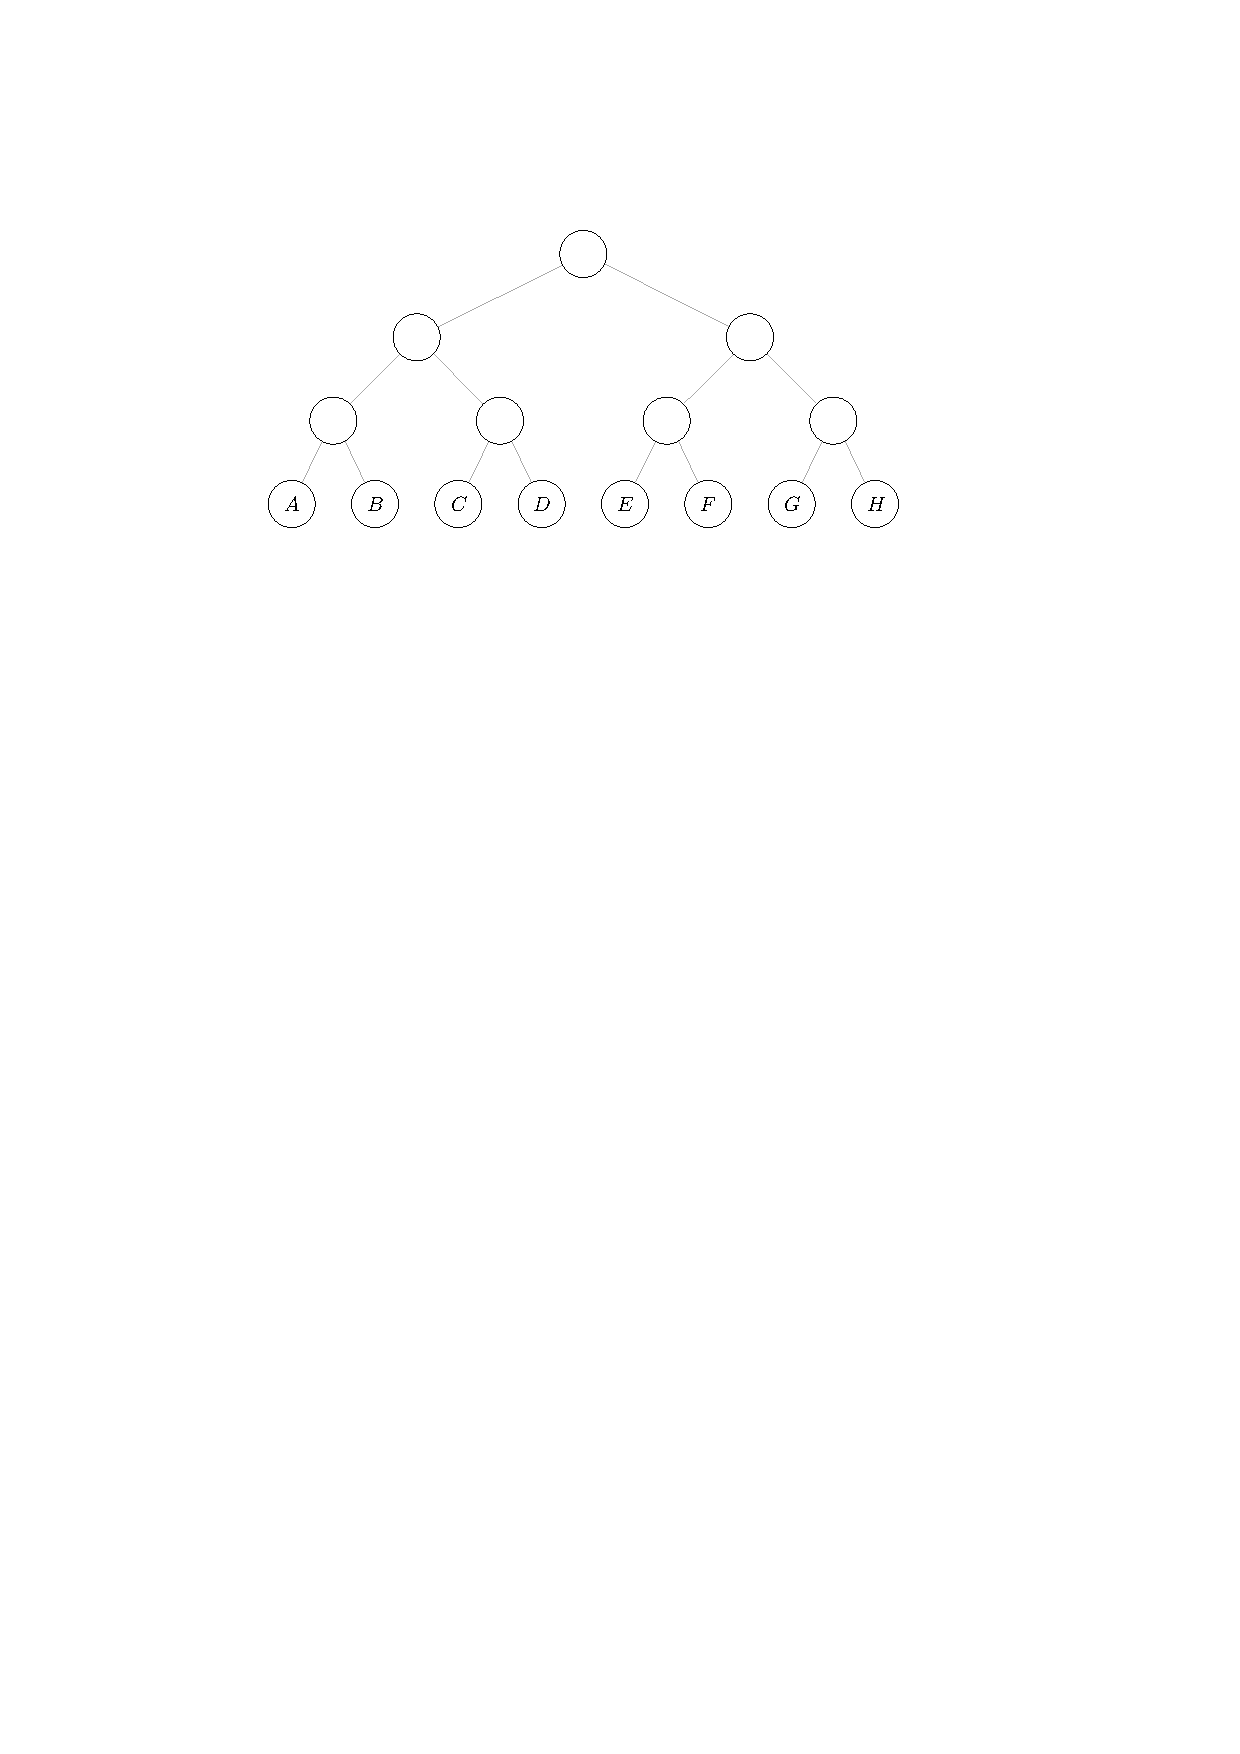
\includegraphics{figures/treekem-tree}
	\end{center}
	\caption{Illustration of a group with users 8 users in the TreeKEM protocol.}\label{fig:treekem-tree}
\end{figure}

The idea behind this tree structure is that it allows for a user creating a commit with a new group key to share the new group key with the group using only a few encryptions, while still updating all the secrets the user knew in the tree in order to recover from a possible compromise (recall that in a PC-CGKA scheme a commit also updates the committer's key material).
To illustrate how a commit is performed and how the new group key is computed, say a user $A$ performs a commit. First we only consider commits without any proposals. TreeKEM specifies two hash functions $\hgen, \hdep \colon \{0, 1\}^{r(\eta)} \to \{0, 1\}^{r(\eta)}$ where $r$ gives the number of bits of randomness used by $\Pi.\gen(1^\eta)$. Let $d = 3$ the depth of user $A$. $A$ will replace all the $d + 1$ nodes on their path to the root (including their leaf) with new nodes $A, p_1, \ldots, p_d$. Although it would be more accurate to say that $A$ just replaces the information stored in the original nodes, and this view makes more sense when implementing the protocol, it will become convenient later to say that $A$ creates new nodes.
The key pairs for the new nodes are sampled as follows. For the leaf node $A$, user $A$ simply samples a key pair by running $\Pi.\gen(1^\eta)$. For the remaining nodes, they first sample $s_1 \from \{0, 1\}^{r(\eta)}$ and compute the key pair of the first parent $p_1$ as $\Pi.\gen(1^\eta, \hgen(s_1))$. For $i \in \{2, \ldots, d\}$ they then compute $s_i \coloneqq \hdep(s_{i - 1})$ and set the key pair of $p_i$ to be $\Pi.\gen(1^\eta, \hgen(s_i))$. The new group key is $k \coloneqq \hdep(s_{d})$.

User $A$ only needs to share (encryptions of) the seeds $s_i$ for the other users to update their view of the tree and compute the new group key:
\begin{itemize}
	\item To share the group key with user $B$, $A$ computes the ciphertext $c_1 \coloneqq \Pi.\enc_{pk_B}(s_1)$. $B$ can then compute the seed $s_1$, then use that to compute the seeds $s_2, \ldots, s_d$, the key pairs of all new nodes on their path to the root and the group key $k$.
	\item To share the new group key with users $C$ and $D$, $A$ computes the ciphertext $c_2 \coloneqq \Pi.\enc_{pk_X}(s_2)$, where $X$ is the parent of the nodes $C$ and $D$. Both $C$ and $D$ know the secret key $sk_X$ of their parent and can decrypt $c_2$.
	\item To share the new group key with users $E, F, G$ and $H$, $A$ computes the ciphertext $c_3 \coloneqq \Pi.\enc_{pk_Y}(s_3)$, where $Y$ is the right child of the root node. Again, all users under $Y$ know $sk_Y$ and can thus decrypt $c_3$.
\end{itemize}
The commit $c$ that $A$ shares with all users includes the ciphertexts $c_1, c_2$ and $c_3$ and the public keys of all new nodes. Figure~\ref{fig:treekem-simple-update} illustrates the commit performed by $A$.

\begin{figure}
	\begin{center}
		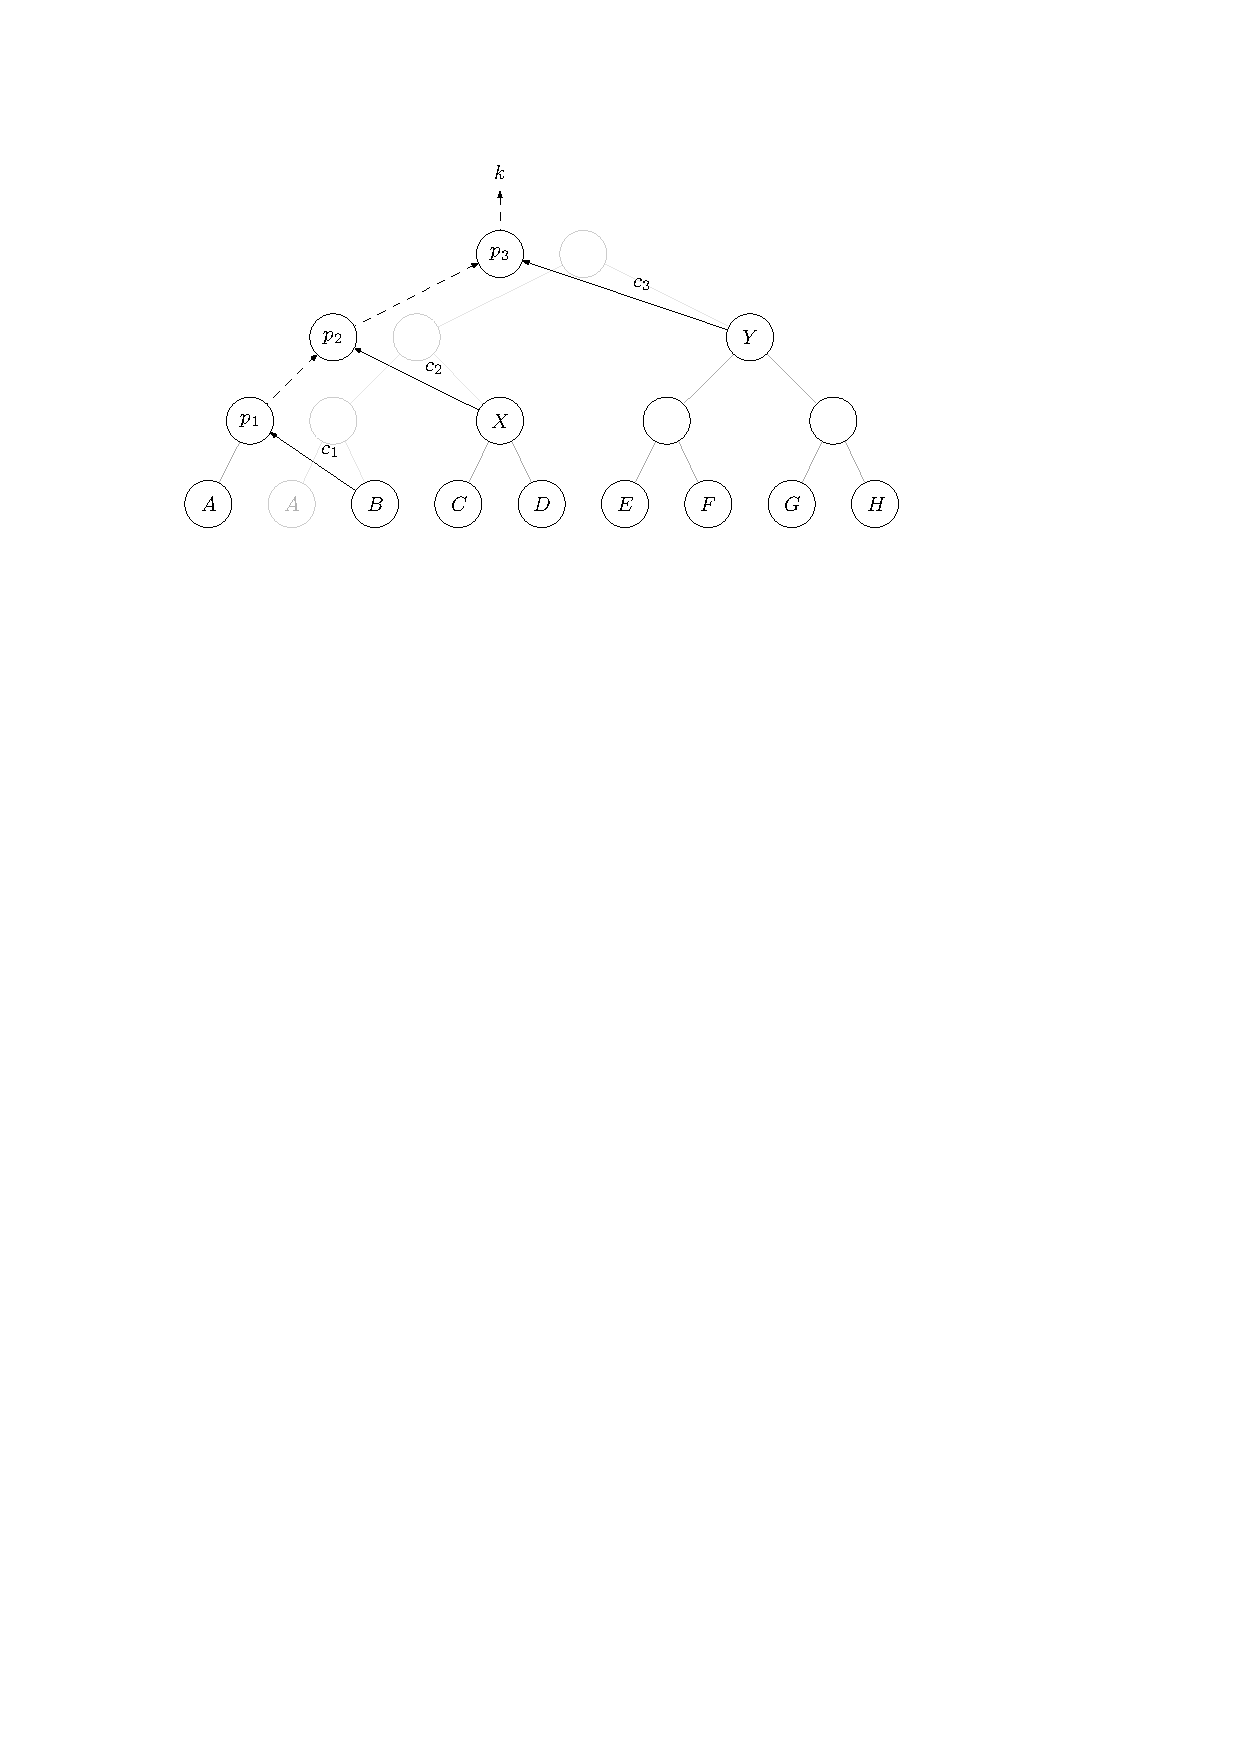
\includegraphics{figures/treekem-simple-update}
	\end{center}
	\caption{The commit by user $A$ described in the text. Dashed directed edges illustrate the fact that the target is related to the source via the hash function $\hdep$. The solid directed edges illustrate the fact that the seed of the target node is encrypted to the public key of the source node.}\label{fig:treekem-simple-update}
\end{figure}

The nodes $B, X$ and $Y$ form the \emph{copath} of $A$: the copath of a node consists of the sibling of each node on the node's path to the root, excluding the root itself. In the ideal case as above, a node performing a commit only has to compute an encryption for each node on it's copath, i.e. logarithmically many in the total number of users.

Things look a bit different if the commit contains a remove proposal. Say user $A$ creates a commit that contains a remove proposal for user $E$. We could just let $A$ replace the nodes on $E$'s direct path $E$ and not encrypt anything for $E$. However, if $A$ were compromised while replacing $E$'s direct path and performed another commit to update their key material after the compromise, the information leaked in the compromise could still be used to compute the new group key, as it includes the secret keys of the nodes on $E$'s direct path.
Instead, all nodes on $E$'s leaf and all nodes on $E$'s direct path are replaced by \emph{blank} nodes: nodes with no associated key pair. Now $A$ would have to encrypt the secret $s_3$ directly to $F$ and to the parent node of $G$ and $H$ in the commit removing user $E$. See Figure~\ref{fig:treekem-remove-user}. A blank leaf node can be populated with a new user. A blank node that is not a leaf will be replaced by a normal node once some user below the node performs a commit. Blank nodes are also useful to represent empty subtrees that have no users.

\begin{figure}
	\begin{center}
		\todo{create figure}
	\end{center}
	\caption{The commit by user $A$ removing user $E$ described in the text.}\label{fig:treekem-remove-user}
\end{figure}

Creating a commit with an update proposal for user $u$ is analogous. The update proposal simply contains the public key of user $u$'s new leaf, while $u$ stored the corresponding secret key locally when creating the proposal. Because we don't want the committer to know the secret keys along $u$'s direct path, we must again blank all these nodes and encrypt to the populated nodes below these blank nodes directly.

Adding a node introduces one more complication. Consider the same group as in Figure~\ref{fig:treekem-tree}, but with the leaf of user $G$ blank. Now say user $A$ would like to add user $G$ to the group.

\todo{Finish explanation of adding a user and unmerged leaves.}

\todo{Define resolution.}

\subsection{Algorithms}

\todo{Describe algorithms.}

% Algorithm $\gen$:
% \begin{itemize}
% 	\item generate init key and private key with $\dhies.\gen$
% 	\item generate leaf node public and private key with $\dhies.\gen$
% 	\item output init key and leaf node public key as public key, and both private keys as secret key
% \end{itemize}
%
% Algorithm $\operatorname{ProposeUpdate}(\sigma)$:
% \begin{itemize}
% 	\item generate $(pk, sk) \dhies.\gen()$
% 	\item output proposal $(pk)$ and store $sk$ in $\sigma$
% \end{itemize}
%
% Algorithm $\operatorname{ProposeAdd}(\sigma, pk_{\mathrm{new}})$:
% \begin{itemize}
% 	\item output proposal $(pk_{\mathrm{new}})$ and store the proposal in $\sigma$
% \end{itemize}
%
% Algorithm $\operatorname{ProposeRemove}(\sigma, v)$:
% \begin{itemize}
% 	\item $v$ is the leaf node of the user to be removed
% 	\item output proposal $(v)$ and store the proposal in $\sigma$
% \end{itemize}

\section{TreeKEM security from SD-GSD security}

\todo{Describe relationship between TreeKEM tree structure and GSD game.}

% To motivate the main result of this section, let us make clear the relation between the PC-CGKA game for TreeKEM and the playing the SD-GSD security game. Consider the tree representing a group in TreeKEM. We can create a matching node in a GSD graph for each node in the tree. Each tree node except the root either has a key pair generated

\todo{Finish statement of Theorem.}

\begin{theorem}
	Let $c, p, u \in \mathbb{N}$. Let $\treekem$ the TreeKEM protocol and recall the hash functions $\hgen, \hdep \colon \{0, 1\}^\lambda \to \{0, 1\}^\lambda$ used in TreeKEM. Let $\dhies$ the DHIES scheme instantiated with a private-key encryption scheme $\Pi_s$. Let $\hdh$ the KDF and $\mathbb{G}$ the group used in $\dhies$. If $\Pi_s$ is $(t, \epsilon)$-EAV secure, the DDH problem is $(t, \epsilon)$-hard in $\mathbb{G}$ and $\hgen, \hdep$ and $\hdh$ are modelled as random oracles, then $\treekem$ is $(\tilde{t}, \tilde{\epsilon}, c, p, u)$-PC-CGKA secure with
	\[
		\tilde{\epsilon} = 2 \cdot (u + 1) \cdot N \cdot \epsilon + \frac{2 \cdot \mdh \cdot N^2}{q} + \frac{\ms \cdot N}{2^{\lambda - 1}},
	\]
	where $N = c \cdot (\lceil \log(u) \rceil + 1) + p$, $\ms$ is an upper bound on the number of queries made to either $\hgen$ or $\hdep$ and $\mdh$ is an upper bound on the number of queries made to $\hdh$, and with
	\[
		\tilde{t} = \ldots
	\]
\end{theorem}

\paragraph{Intuition} \todo{provide outline of the proof and reference proof in \cite{modular-group-messaging}.}
